\documentclass[sans]{beamer}

% \usetheme{Boadilla}
\mode<presentation>
{
	% \usetheme{CambridgeUS}
	\usetheme{AnnArbor}
	% \usetheme{Bergen}
	\usecolortheme{beaver}
	% \usefonttheme{serif}
	% \usefonttheme{professionalfonts}
	% \usefonttheme{structureitalicserif}
}

\usepackage{cmap}
\usepackage{listings}
\usepackage{lmodern}
\usepackage{color}
\usepackage{minted}
\usepackage{graphicx}
\usepackage{tikz}
\usepackage{wrapfig}

% \usepackage[labelformat=empty]{subcaption}
\usepackage[labelformat=empty]{caption}

% \usefonttheme{professionalfonts} % using non standard fonts for beamer
% \usefonttheme{sansserif} % default family is serif
% \usepackage{fontspec}
% \usepackage[T2A]{fontenc}
% \setmainfont{Comic Sans MS}

% \usepackage[utf8]{inputenc}
% \usepackage[russian]{babel}

\usepackage{fontspec}
% \setmainfont[Mapping=tex-text]{CMU Serif}



\usepackage{polyglossia}
\setdefaultlanguage{russian}

% \newfontfamily\cyrillicfont[Script=Cyrillic]{Comic Sans MS}
% \newfontfamily{\cyrillicfontt} {Comic Sans MS}
% \newfontfamily{\cyrillicfonttt}{Comic Sans MS}

\setmainfont[Ligatures=TeX]{DejaVu Serif}
\setsansfont[Ligatures=TeX]{DejaVu Sans}
% \setmainfont[Ligatures=TeX]{Comic Sans MS}
% \setsansfont[Ligatures=TeX]{Comic Sans MS}
\setmonofont{DejaVu Sans Mono}

% \setmathfont{XITS Math}
% \defaultfontfeatures{Scale=MatchLowercase,Mapping=tex-text}

\begin{document}

\title[Форматирование по эталону] {Форматирование по эталону}
% \subtitle {Летняя стажировка}
% \institute {JetBrains, СПбГУ}

\institute{JetBrains, СПбГУ \\
	\vspace{0.7cm}
	Руководитель: к.ф.-м.н. Булычев Д.Ю.
	\vspace{0.7cm}	
}


\author
[Подкопаев Антон]{Подкопаев Антон, \texttt podkoav239@gmail.com}
\date [27-09-13]{27 сентября 2013}

\begin{frame}[plain]
	\titlepage
\end{frame}

\section{Описание контекста задачи}

\begin{frame}{Печать AST}
	% \begin{center}
	
\includegraphics[height = 3cm]{images/tree.jpg}
	% \hspace{0.5cm}
	\begin{figure}
		
\includegraphics[width = 2cm]{images/arrow.png}
	\end{figure}
	% \hspace{0.5cm}

	\hfill
	
\includegraphics[height = 3cm]{images/text.png}
	% \end{center}
\end{frame}

\begin{frame}{Область применения}
	Языковые процессоры
	\begin{itemize}
		\item Синтаксический анализ
		\item Преобразование
		\item Представление результата
		% Часто результат - программа на другом языке
		\begin{itemize}
			\item \textcolor{red}{Код программы}
			\item ...
		\end{itemize}
	\end{itemize}
\end{frame}

\begin{frame}{Печать AST с помощью шаблонов}
	\begin{itemize}
		\item Модельный язык L
		\item Специальные шаблоны
		\item Расширенный парсер
		\item Сопоставление деревьев сверху-вниз
		\begin{itemize}
			\item $O(T \times B \times M)$
		\end{itemize}
	\end{itemize}
	\begin{block}{}
		\inputminted{pascal}{codes/l_write.t}
	\end{block}
\end{frame}

% \begin{frame}{Печать AST с помощью шаблонов. Алгоритм}
% 	\begin{itemize}
% 		\item 
% 		\item $O(T \times B \times M)$
% 		\begin{itemize}
% 			\item T --- размер дерева
% 			\item B --- максимальный размер образца
% 			\item M --- количество образцов
% 		\end{itemize}
% 	\end{itemize}
% \end{frame}

\section{Постановка задачи}

\begin{frame}{Постановка задачи}
	\begin{itemize}
		\item Апробирование для Java
		\item Плагин для IDEA
		\item Алгоритм, перебирающий все подходящие шаблоны
	\end{itemize}
	\pause
	\begin{itemize}
		\item Отказ от специализированного парсера
		\item Получение шаблонов из обычных исходников
	\end{itemize}
\end{frame}

\begin{frame}{}
	\begin{columns}[T]
		\begin{column}{.5\textwidth}
			\begin{figure}
				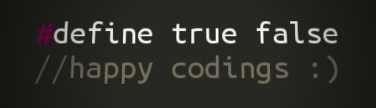
\includegraphics[width = \linewidth]{images/trueFalse.png}
				\caption{Эталон}
			\end{figure}
			\begin{figure}
				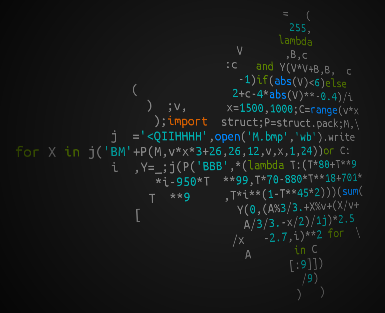
\includegraphics[height = 3cm, width = \linewidth]{images/mandel.png}
				\caption{Для переформатирования}
			\end{figure}
		\end{column}

		\pause

		\begin{column}{.5\textwidth}
			\begin{minipage}[c][0.8\textheight][c]{\linewidth}
				\begin{figure}[c]
					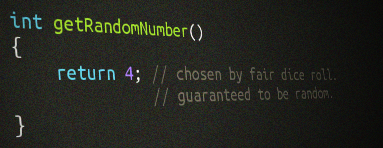
\includegraphics[width = \linewidth]{images/rand.png}
					\caption{Результат}
				\end{figure}
			\end{minipage}

		\end{column}
	\end{columns}
\end{frame}

% \begin{frame}{Существующие решения}
% 	
\includegraphics[width = \linewidth]{images/quiz_night.jpg}
% \end{frame}

% \begin{frame}{Инструменты}
% 	\begin{center}
% 		
\includegraphics[width = 0.3\linewidth]{images/idea-logo.png}
% 		\hspace{3cm}
% 		
\includegraphics[width = 0.3\linewidth]{images/kotlin-logo.jpg}
% 	\end{center}
% \end{frame}

\section{Решение задачи}

\begin{frame}{Трудности}
	\begin{itemize}
		\item Вырезка шаблонов
		\item Комментарии
		\item Экспонента в списках и бинарных выражениях
		\begin{itemize}
			\item Фиксированные варианты
		\end{itemize}
	\end{itemize}

	\begin{itemize}
		\item Требуется большой эталон 
		\item Несколько стилей в эталоне
		\item Экспоненциальность алгоритма
		\begin{itemize}
			\item Локальный выбор 
		\end{itemize}
	\end{itemize}
\end{frame}

% \begin{frame}{Комментарии}
	
% \end{frame}

\section{Будущее развитие}

\begin{frame}{В будущем}
	\begin{itemize}
		\item Нормализация шаблонов
		\item Анализ эталона на полноту
		\item Сохранение пользовательского форматирования?
		\item Интеграция с Formatter?
		\item Машинное обучение?
	\end{itemize}
\end{frame}

\section{Результат}

\begin{frame}{Результат}
	\begin{itemize}
		\item Прототип плагина
			\newline
			\color{blue}\underline{\url{bitbucket.org/anlun/printerplugin}}
			\color{black}
		\item Расширен общий подход
	\end{itemize}
\end{frame}

\appendix

\begin{frame}{Можно ли проще?}
	% \pause
	Вообще-то да...
	\newline

	\begin{columns}
		\begin{column}{.4\textwidth}
			\begin{figure}
				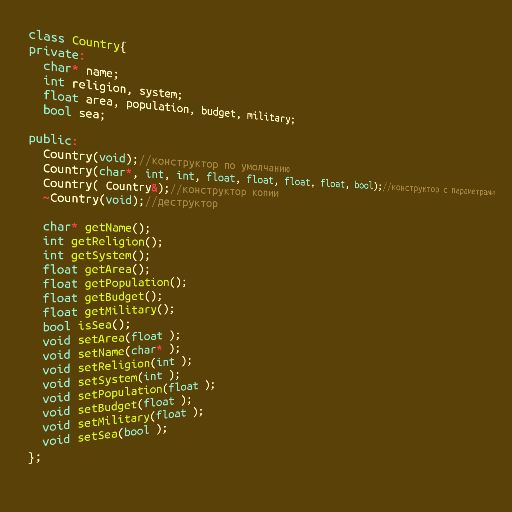
\includegraphics[width = \linewidth]{images/country.png}
			\end{figure}
		\end{column}

		\begin{column}{.1\textwidth}
			\begin{figure}
				
\includegraphics[width = \linewidth]{images/arrow.png}
			\end{figure}
		\end{column}

		\begin{column}{.4\textwidth}
			\begin{figure}
				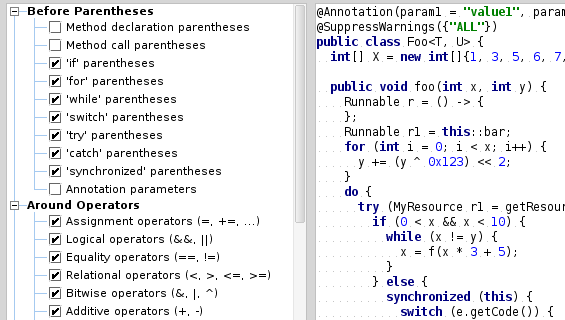
\includegraphics[width = \linewidth]{images/snapshot1.png}
			\end{figure}
		\end{column}
	\end{columns}
\end{frame}

\end{document}